%!TEX program = xelatex
\documentclass[12pt,a4paper,utf8]{ctexart}
\usepackage{graphicx}
\usepackage{amsmath}
\usepackage{amssymb}
\usepackage{subfig}
\usepackage{cite}
\usepackage[ntheorem]{empheq}
\usepackage{enumitem}
\usepackage{fullpage}
\usepackage{cleveref}
\usepackage{cellspace}
\usepackage{listings}
\usepackage{color}
\definecolor{gray}{rgb}{0.5,0.5,0.5}
\definecolor{dkgreen}{rgb}{.068,.578,.068}
\definecolor{dkpurple}{rgb}{.320,.064,.680}

% set Matlab styles
\lstset{
   language=Matlab,
   keywords={break,case,catch,continue,else,elseif,end,for,function,
      global,if,otherwise,persistent,return,switch,try,while},
   basicstyle=\ttfamily,
   keywordstyle=\color{blue}\bfseries,
   commentstyle=\color{dkgreen},
   stringstyle=\color{dkpurple},
   backgroundcolor=\color{white},
   tabsize=4,
   showspaces=false,
   showstringspaces=false
}

\begin{document}
\CJKfamily{zhkai}	


\begin{center}
\textbf{作业三}\\
\textbf{林成渊 ~~~~~ PB18051113 ~~~~~ \zhtoday}\\
\end{center}
\textit{}
\vspace{\baselineskip}

\begin{enumerate}
\item[第一题] \textbf{本题考虑对称矩阵的Gauß消去法和LU分解}

(a)假设$ A $是一个满足$ a_11 \neq 0 $的对称矩阵,当$ A $的第一列完成消去的时候我们得到
\begin{equation}
	\left[\begin{matrix}
		a_{11} & a_{12}\dots a_{1n} \\
		0 &  \\
		\vdots & A^{(1)}\\
		0 & 
	\end{matrix}\right] \nonumber
\end{equation}
证明$ A^{(1)} $是对称的。

证明:设$ A = \{a_{ij}\}_{n\times n} ,\quad A^{(1)} = \{a'_{ij}\}_{(n-1)\times (n-1)}$,由$ a_11 \neq 0 $,那么根据消去规则有
\begin{equation}
	\begin{aligned}
		(0,a'_{11},a'_{12},\dots ,a'_{1(n-1)}) &= (a_{21},a_{22},\dots ,a_{2n}) - \frac{a_{21}}{a_{11}} (a_{11},a_{12},\dots , a_{1n}) \\
			&= (0,a_{22} - \frac{a_{21}}{a_{11}})a_{12},\dots ,a_{2n} - \frac{a_{21}}{a_{11}} a_{1n})
	\end{aligned}
	\nonumber
\end{equation}
同理有,对$ \forall i,j \in N^* $,
\begin{equation}
	a'_{ij} = a_{(i+1)(j+1)} - \frac{a_{(i+1)1}}{a_{11}}a_{1(j+1)} \nonumber
\end{equation}
$ \because A$为正定矩阵,$ \forall i,j \in N^*, a_{ij} = a_{ji} $,则对于$ A^{(1)} $有
\begin{equation}
	\begin{aligned}
		a'_{ji} &= a_{(j+1)(i+1)} - \frac{a_{(j+1)1}}{a_{11}} a_{1(i+1)} \\
				&= a_{(i+1)(j+1)} - \frac{a_{(i+1)1}}{a_{11}} a_{1(j+1)} \\
				&= a'_{ij}
	\end{aligned}
	\nonumber
\end{equation}
$ \therefore A^{(1)}$是对称的



(b)根据上一问的结论用伪代码的形式写出计算一个正定矩阵$ LU $分解的算法,利用对称性节省计算量。

算法思路: 

由于是对称正定矩阵,故其在每一轮高斯消元时都能保证$ a_{ii} \neq 0$(见《Linear Algebra with Applications(9th Edition)》--Steven J.Leon).由于每次消元的子矩阵都是对称的,故只需算出其上三角部分,下三角部分直接对称赋值即可,节约计算量。

算法伪代码:
\begin{lstlisting}[frame=single]
% 对正定对称矩阵A进行不做行交换的LU分解.
[sx,sy] = size(A);
U = A;
L = zeros(sx,sy);
for i = 1 : sy
	L(i,i) = 1;
	for j = i + 1 : sx
		L(j,i) = U(j,i) / U(i,i);
		U(j,i) = 0;
		for k = j : sy
			U(j,k) = U(j,k) - L(j,i) * U(i,k);
			U(k,j) = U(j,k);
		end
	end
end
\end{lstlisting}

(c)编写程序,用Cholesky分解解给定方程组$ Ax = b $。

代码如下
\begin{lstlisting}[frame=single]
clear, clc

A = [4,-2,4,2;-2,10,-2,-7;4,-2,8,4;2,-7,4,7];
b = [8;2;16;6];
showAb(A,b);
% 对正定对称矩阵A进行不做行交换的LU分解.
[sx,sy] = size(A);
U = A;
L = zeros(sx,sy);
for i = 1 : sy
	L(i,i) = 1;
	for j = i + 1 : sx
		L(j,i) = U(j,i) / U(i,i);
		U(j,i) = 0;
		for k = j : sy
			U(j,k) = U(j,k) - L(j,i) * U(i,k);
			U(k,j) = U(j,k);
		end
	end
end
showLU(L,U);
%对L进行行列数乘得到新的L,即Cholesky分解
for i = 1 : sx
	factor = sqrt(U(i,i));
	for j = i : sx
		L(j,i) = L(j,i) * factor;
	end
end
showLLt(L,L');
%根据L求解Y
Y = zeros(sy,1);
for i = 1 : sy
	Y(i) = b(i);
	for j = 1 : i - 1
		Y(i) = Y(i) - L(i,j) * Y(j);
	end
	Y(i) = Y(i) / L(i,i);
end
%根据L的转置求解X
X = zeros(sx,1);
for i = sy : -1 : 1
X(i) = Y(i);
for j = i + 1 : sx
X(i) = X(i) - L(j,i) * X(j);
end
X(i) = X(i) / L(i,i);
end
%输出解
fprintf("x = \n");
disp(X);
%%
%输出A和b
function showAb(A,b)
% Display the matrix A and the vector b
%	used in Gauss elimination
...此处省略
end
%%
%输出L和U
function showLU(L,U,varargin)
% Display the matrix L and U
%	got in LU decomposition
...此处省略
end
%%
%输出L和L'
function showLLt(L,Lt,varargin)
% Display the matrix L and U
%	got in LU decomposition
...此处省略
end

\end{lstlisting}
输出结果如图1
\begin{figure}[htbp]
    \centering
    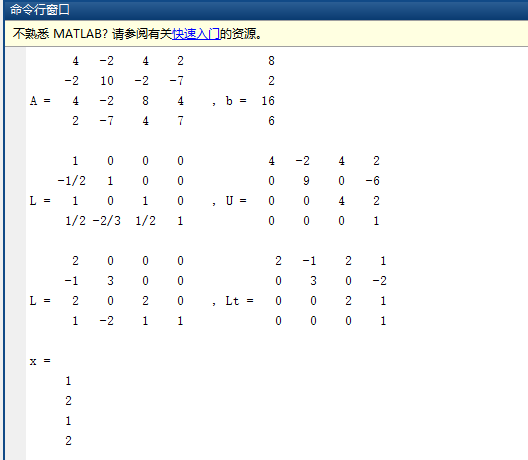
\includegraphics[width=0.6\textwidth]{image/T1_c.png}
    \caption{第一题(c)小题结果}
\end{figure}

\item[第二题] \textbf{Richardson迭代方法},对于通用迭代格式
\begin{equation}
	x^{(k+1)} = M^{-1} Nx^{(k)}+M^{-1}b \nonumber
\end{equation}
Richardson迭代的$ M = \frac{1}{\omega} I$,$ N=\frac{1}{\omega}I - A$,此处$ \omega > 0 $。考虑$ A $为正定的情况,并设$ A $的最小和最大特征值分别为$ \lambda_1 $和$ \lambda_n $

(a)证明Richardson迭代方法在$ \omega < \frac{2}{\lambda_n} $的情况下收敛

证明:由
\begin{equation}
	x^{(k+1)} = M^{-1} Nx^{(k)}+M^{-1}b \nonumber
\end{equation}
有
\begin{equation}
	Mx^{(k+1)} = Nx^{(k)}+b \nonumber
\end{equation}
代入精确值(代入$ k\rightarrow \infty $)后与原式相减得到
\begin{equation}
	M(x^{(k+1)}-x) = N(x^{(k)}-x) \nonumber
\end{equation}
令误差$ e^{k} = |x^{k} - x |$有
\begin{equation}
	Me^{(k+1)} = Ne^{(k)} \nonumber
\end{equation}
即
\begin{equation}
	e^{(k+1)} = (I-\omega A)e^{(k)} \nonumber
\end{equation}
如此,考察矩阵$ G = I - \omega A $的特征值,设由$ A $的特征值构成的对角矩阵为$ D_A $,于是
\begin{equation}
	\begin{aligned}
		I - \omega A &= I - \omega P^{-1}D_AP \\
					&= P^{-1}IP - P^{-1}\omega D_AP \\
					&= P^{-1} (I - \omega D_A)P \\
					&= P^{-1} D_{I-\omega A} P
	\end{aligned}
	\nonumber
\end{equation}
所以$ G $的谱半径$ \rho(G_{\omega }) $,即$ G $的特征值的绝对值最大值为$ max|1-\omega \lambda_i| $,而由题意,在$ \omega < \frac{2}{\lambda_n} $的时候
\begin{equation}
	\begin{aligned}
		\rho(G_{\omega }) & = max|1-\omega \lambda_i| \\
						& = max\{|1-\omega \lambda_1| , |1-\omega \lambda_n| \} \\
						& < 1
	\end{aligned}
	\nonumber
\end{equation}
所以Richardson迭代方法在该条件下收敛

(b)证明其谱半径以及取最佳值时候的$ \omega $值

由等式
\begin{equation}
	1-\omega \lambda_1 = \omega \lambda_n -1 \nonumber
\end{equation}
解得$ \omega = \frac{2}{\lambda_1+\lambda_n} $,记作$ \omega_b $
引用上一小题结论有
\begin{equation}
	\begin{aligned}
		\rho(G_{\omega }) & = max\{|1-\omega \lambda_1| , |1-\omega \lambda_n| \} \\
						& = \left\{\begin{aligned}
								& 1 - \omega \lambda_1\quad &,\omega \le \omega_b \\
								&\frac{\lambda_n - \lambda_1}{\lambda_n+\lambda_1}\quad &,\omega = \omega_b \\
								&\omega \lambda_n - 1\quad &,\omega \ge \omega_b
							\end{aligned}\right.
	\end{aligned}
	\nonumber
\end{equation}
易证其取到最小值的时候,即最优情况下,$ \omega = \omega_b = \frac{2}{\lambda_1+\lambda_n}$.


(c)设计一个方法用Matlab随机数生成函数rand构造出2一个5×5的特征值为1, 2, 3, 4, 5的正定矩阵作为A,再用rand构造出一个5 × 1的向量作为b。然后用上述Richardson迭代方法解Ax = b,作图验证收敛半径。

代码如下
\begin{lstlisting}[frame=single]
clear, clc

P = orth(rand(5,5));
B = diag([1,2,3,4,5]);
A = P\B*P;
b = rand(5,1);
F = @(x) (x > 2/(1+5)) .* (5 * x - 1) + (x <= 2/(1+5)) .* (1 - x);
%%
%遍历
wstep = 1e-3;
wnum = 2/5 /wstep;
wSet = linspace(wstep,2/5-wstep,wnum-1);
rhoReal = F(wSet);
rhoSet = zeros(wnum-1,1);
for i = 1 : wnum-1
	G = eye(5)-wSet(i)*A;
	x_next=zeros(5,1);
	e_next = 1;
	while(e_next>1e-11)
		x_curr = x_next;
		x_next = G*x_curr+wSet(i)*b;
		e_curr = e_next;
		e_next = norm(x_next-x_curr);
	end
	rhoSet(i) = e_next/e_curr;
end

%%
%计算rho
wBest = 2/(1+5);
G = eye(5)-wBest*A;
while(norm(x_next-x_curr)>1e-11)
	x_curr = x_next;
	x_next = G*x_curr+wBest*b;
end
fprintf("x=\n");
disp(x_next);

%%
%绘图验证

figure(1);
p1 = plot(wSet,rhoSet,'k'); hold on
p2 = plot(wSet,rhoReal,'b'); hold on
legend ([p1 ,p2], 'approx ', 'real');
xlabel('omega');
ylabel('rho');

%%
%输出A和b
function showAb(A,b)
% Display the matrix A and the vector b
%	used in Gauss elimination
...此处省略
end
%%
%输出L和U
function showLU(L,U,varargin)
% Display the matrix L and U
%	got in LU decomposition
...此处省略
end
%%
%输出L和L'
function showLLt(L,Lt,varargin)
% Display the matrix L and Lt
%	got in LU decomposition
...此处省略
end
\end{lstlisting}
运行输出绘图结果如图2,可见和表达式基本吻合。计算得到方程解如图3.
\begin{figure}[htbp]
	\centering
	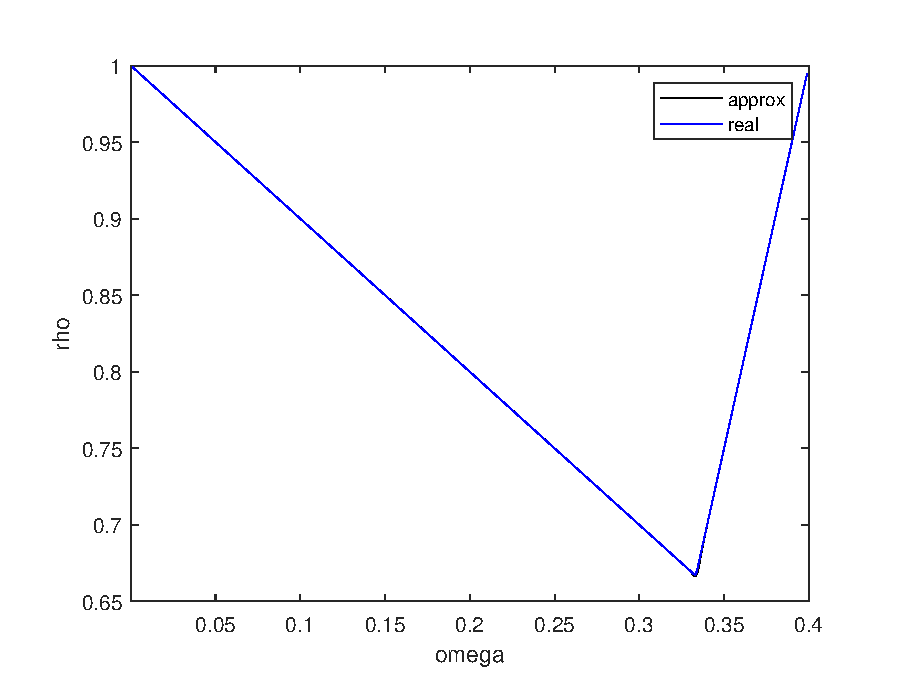
\includegraphics[width=0.6\textwidth]{image/T2_c_1.eps}
	\caption{第二题(c)小题作图}
\end{figure}
\begin{figure}[htbp]
	\centering
	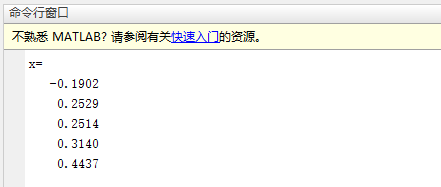
\includegraphics[width=0.6\textwidth]{image/T2_c_2.png}
	\caption{第二题(c)小题方程组解}
\end{figure}

\item[第三题] \textbf{从另一个角度考虑Gauβ积分}

(a)由于高斯积分可以用$ n $个采样点上的采样值精确求得一个$ 2n-1 $阶多项式的定积分.
现取$ n = 6 $,那么可以精确求得任意一个11阶多项式的定积分,
定义一组基函数$ \{1,x,x^2,\dots ,x^11\} $,
设积分结点为$ \{x_i|1\le i \le 12,x_1 < x_2 < \dots < x_{12}\} $,有
\begin{equation}
	\left\{\begin{aligned}
			\quad &\sum_{i=1}^{6} \omega_ix_i^0-2 &= 0 \\
			\quad &\sum_{i=1}^{6} \omega_ix_i^1-\frac{0}{2} &= 0 \\
			\quad &\sum_{i=1}^{6} \omega_ix_i^2-\frac{2}{3} &= 0 \\
			\quad &\ldots &\\
			\quad &\sum_{i=1}^{6} \omega_ix_i^{11}-\frac{0}{12} &= 0
		\end{aligned}\right.
	\nonumber
\end{equation}
又由积分结点和积分权重关于原点的对称性,原方程组简化为(此处只需在意结点的排布顺序,哪边更大并不影响)
\begin{equation}
	\left\{\begin{aligned}
		\quad &\sum_{i=1}^{3} \omega_i x_i^0-1 &= 0 \\
		\quad &\sum_{i=1}^{3} \omega_i x_i^2-\frac{1}{3} &= 0 \\
		\quad &\ldots &\\
		\quad &\sum_{i=1}^{3} \omega_i x_i^{10}-\frac{1}{11} &= 0 \\
		\quad &x_1 + x_6 &= 0 \\
		\quad &x_2 + x_5 &= 0 \\
		\quad &x_3 + x_4 &= 0 \\
		\quad &\omega_1 - \omega_6 &= 0 \\
		\quad &\omega_2 - \omega_5 &= 0 \\
		\quad &\omega_3 - \omega_4 &= 0 \\
		\quad &x_1^2,x_2^2,x_3^2 &> 0
	\end{aligned}\right.
	\nonumber
\end{equation}
将$ x_i^2 $视作一个变量$ s_i $,方程式变为
\begin{equation}
	\left\{\begin{aligned}
		\quad &\sum_{i=1}^{3} \omega_is_i^0-1 &= 0 \\
		\quad &\sum_{i=1}^{3} \omega_is_i^1-\frac{1}{3} &= 0 \\
		\quad &\ldots &\\
		\quad &\sum_{i=1}^{3} \omega_is_i^5-\frac{1}{11} &= 0 \\
		\quad &s_1,s_2,s_3 &> 0
	\end{aligned}\right.
	\nonumber
\end{equation}

(b)直接求导写出其雅可比矩阵
\begin{equation}
	\left[\begin{array}{cccccc}
		0 & 0 & 0 & 1 & 1 & 1 \\
		 \omega_1 		&  \omega_2 		&  \omega_3 		& s_1 	& s_2 	& s_3 \\
		2\omega_1 s_1	& 2\omega_2 s_2		& 2\omega_3 s_3		& s_1^2 & s_2^2 & s_3^2 \\
		3\omega_1 s_1^2	& 3\omega_2 s_2^2	& 3\omega_3 s_3^2	& s_1^3 & s_2^3 & s_3^3 \\
		4\omega_1 s_1^3	& 4\omega_2 s_2^3	& 4\omega_3 s_3^3	& s_1^4 & s_2^4 & s_3^4 \\
		5\omega_1 s_1^4	& 5\omega_2 s_2^4	& 5\omega_3 s_3^4	& s_1^5 & s_2^5 & s_3^5
	\end{array}\right]
	\nonumber
\end{equation}

(c)选取等距节点$ \{x_i\} = \{-1,-0.6,-0.2,0.2,0.6,1\} $,转化为$ \{s_i\} = \{0.04,0.36,1\}$.

观察积分权重公式
\begin{equation}
	\int_{-1}^1 \frac{\prod_{k \neq i} (x - x_k)}{\prod_{k \neq i} (x_i - x_k)} dx\nonumber
\end{equation}
其被积函数在除了$ x_i $之外的所有插值点其值都为0,由于其本身是一个多项式函数,所以对其可以粗略看成仅在$ x_i $附近的两个点之间对积分做了主要贡献,由于插值点均匀分布,那么其对于在每个插值点上的权重积分便具有粗糙的对称性,换言之所有权重趋向于值相近,而贡献总和由方程组的第一个方程可以粗略估计为$ 2 $,故最终确定权值为各个点均分$ 2 $。
\begin{lstlisting}[frame=single]
clear, clc

n = 6;
X_curr = [0,0,0,0,0,0]';
X_next = [0.04,0.36,1,0.33,0.33,0.33]';
err_past = 3;
err_curr = 2;
err_next = 1; 
DF = zeros(6,6);
n = 1;
while(norm(X_next-X_curr)>1e-7)

	X_curr = X_next;
	%构造DF
	fprintf("n=");
	disp(n);
	n = n + 1;	
	DF(1,:) = [0,0,0,1,1,1];
	DF(2,:) = [X_curr(4:6)',X_curr(1:3)'];
	DF(3,:) = DF(2,:) .* [X_curr(1:3)',X_curr(1:3)'];
	DF(4,:) = DF(3,:) .* [X_curr(1:3)',X_curr(1:3)'];
	DF(5,:) = DF(4,:) .* [X_curr(1:3)',X_curr(1:3)'];
	DF(6,:) = DF(5,:) .* [X_curr(1:3)',X_curr(1:3)'];
	DF(3,1:3) = DF(3,1:3) * 2;
	DF(4,1:3) = DF(4,1:3) * 3;
	DF(5,1:3) = DF(5,1:3) * 4;
	DF(6,1:3) = DF(6,1:3) * 5;

	%求解F(x)
	L1 = zeros(6,3);
	U1 = X_curr(4:6)';
	Fx = zeros(6,1);
	L1(1,:) = [1,1,1];
	for i = 2 : 6	
	L1(i,:) = L1(i-1,:) .* X_curr(1:3)';
end
Fx = L1 * U1'-[1,1/3,1/5,1/7,1/9,1/11]';
%迭代求解
X_next = X_curr - DF\Fx;
err_past = err_curr;
err_curr = err_next;
err_next = norm(X_next-X_curr);
p = log(err_curr/err_next)/log(err_past/err_curr);
fprintf("p = ");
disp(p);
end

\end{lstlisting}
运行输出结果如图4和图5
\begin{figure}[htbp]
	\centering
	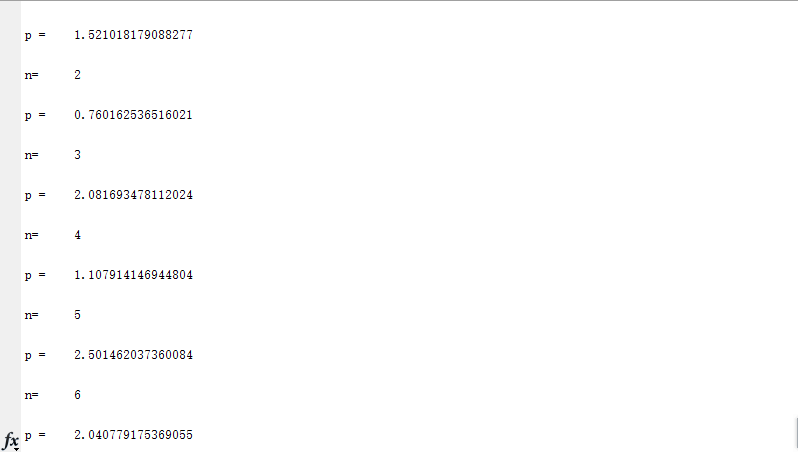
\includegraphics[width=0.6\textwidth]{image/T3_c_1.png}
	\caption{第三题(c)小题迭代次数与收敛阶数}
\end{figure}
\begin{figure}[htbp]
	\centering
	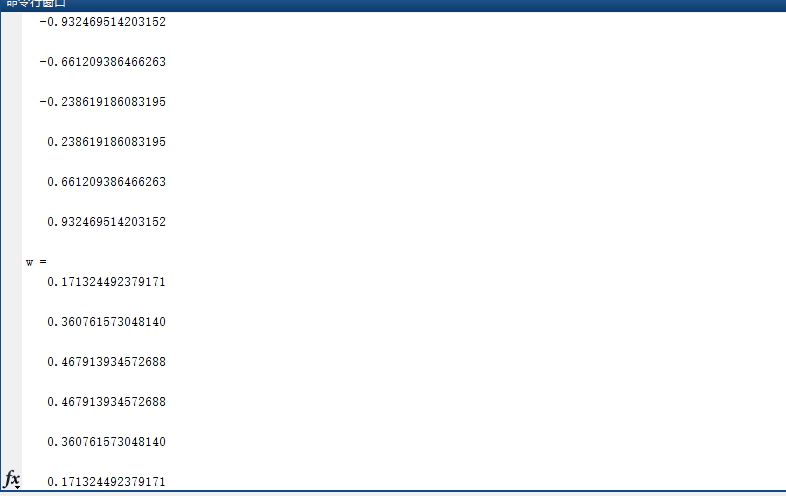
\includegraphics[width=0.6\textwidth]{image/T3_c_2.png}
	\caption{第三题(c)小题解}
\end{figure}

(d)同理先列出其表达式
\begin{equation}
	\begin{aligned}
		\omega_i &= \int_{-1}^1 \frac{\prod_{k \neq i} (cos\frac{x \pi}{n} - cos\frac{k\pi }{n})}{\prod_{k \neq i} (cos\frac{i \pi}{n} - cos\frac{k\pi }{n})} dx \\
		&= \int_{-1}^1 \frac{\prod_{k \neq i} (sin\frac{(x+k) \pi}{2n}sin\frac{(x-k)\pi }{2n})}{\prod_{k \neq i} (sin\frac{(i+k) \pi}{2n}sin\frac{(i-k)\pi }{2n})} dx
	\end{aligned}
	\nonumber
\end{equation}
由其乘积式估得,其赋予均值的估计是合理的。

\begin{lstlisting}[frame=single]
clear,clc

for n = 4 : 30
[realx,realw] = gauss(n);
ns = n-round(n/2);
ChewbyX = linspace(0,n-1,n);
ChewbyPoint = cos(ChewbyX * pi / (n-1)); 
X_next = [ChewbyPoint(1:ns),ones(1,round(n/2))/round(n/2)];
s = ones(n,1);
while (norm(s) > 1e-7)
	X_curr = X_next;
	DF = zeros(n);
	Fx = zeros(n,1);
	if (rem(n,2) == 1)
		[Fx,DF] = SingleDF(ns,X_curr);
	else
		[Fx,DF] = DoubleDF(ns,X_curr);
	end
	s = -inv(DF)*Fx';
	X_next = X_curr + s';
end
if(norm(X_next- 
			[abs(realx(1:n-round(n/2))'),
			realw(1:round(n/2))])>1e-7)
	break;
end
disp(n);
end

%%
function [Fx,DF] = DoubleDF(ns,X)
	Fx = zeros(2*ns,1);
	DF(1,:)  = [zeros(1,ns),ones(1,ns)];
	Fx(1) = sum(X(ns+1:2*ns))-1;
	DF(2,1:ns)  = 2*[X(1:ns) .* X(ns+1:2*ns)];
	DF(2,ns+1:2*ns) = X(1:ns) .* X(1:ns);
	Fx(2) = sum( X(ns+1:2*ns).* DF(2,ns+1:2*ns) ) - 1/3;
	for i = 1 : 2 * ns - 2
		DF(i+2,1:ns) = (i+1)/i * DF(i+1,1:ns) 
						.* DF(2,ns+1:2*ns);
		DF(i+2,ns+1:2*ns) = DF(i+1,ns+1:2*ns) 
							.* DF(2,ns+1:2*ns);
		Fx(i+2) = sum(X(ns+1:2*ns) 
				.*DF(i+2,ns+1:2*ns))-1/(2*i+3);
	end
	Fx = Fx';
end
%%
function [Fx,DF] = SingleDF(ns,X)
	DF(1,:)  = [zeros(1,ns),ones(1,ns),1/2];
	Fx(1) = sum(X(ns+1:2*ns))+X(2*ns+1)/2-1;
	DF(2,1:ns)  = 2*[X(1:ns) .* X(ns+1:2*ns)];
	DF(2,ns+1:2*ns) = X(1:ns) .* X(1:ns);
	Fx(2) = sum(X(ns+1:2*ns).*DF(2,ns+1:2*ns))-1/3; 
	for i = 1 : 2 * ns - 1
		DF(i+2,1:ns) = (i+1)/i * DF(i+1,1:ns) 
							.* DF(2,ns+1:2*ns);
		DF(i+2,ns+1:2*ns) = DF(i+1,ns+1:2*ns) 
							.* DF(2,ns+1:2*ns);
		Fx(i+2) = sum(X(ns+1:2*ns) 
							.*DF(i+2,ns+1:2*ns))-1/(2*i+3);
	end
end

%%
function [X] = LUC(A,b)

% 对正定对称矩阵A进行不做行交换的LU分解.
[sx,sy] = size(A);
	U = A;
	L = zeros(sx,sy);
	for i = 1 : sy
		L(i,i) = 1;
		for j = i + 1 : sx
			L(j,i) = U(j,i) / U(i,i);
			U(j,i) = 0;
			for k = i+1 : sy
				U(j,k) = U(j,k) - L(j,i) * U(i,k);
				%U(k,j) = U(j,k);
			end
		end
	end
	%根据L求解Y
	Y = zeros(sy,1);
	for i = 1 : sy
		Y(i) = b(i);
		for j = 1 : i - 1
			Y(i) = Y(i) - L(i,j) * Y(j);
		end
	end
	%根据U求解X
	X = zeros(sx,1);
	for i = sy : -1 : 1
			X(i) = Y(i);
		for j = i + 1 : sx
			X(i) = X(i) - U(i,j) * X(j);
		end
		X(i) = X(i) / U(i,i);
	end
end

%%
function [x,w] = gauss(N)
	beta = .5./sqrt(1-(2*(1:N-1)).^(-2));
	T = diag(beta,1) + diag(beta,-1);
	[V,D] = eig(T);
	x = diag(D); [x,i] = sort(x);
	w = 2*V(1,i).^2;
end
\end{lstlisting}
运行程序输出结果如图2,可见在该初值选取下最大的n是10.
\begin{figure}[htbp]
	\centering
	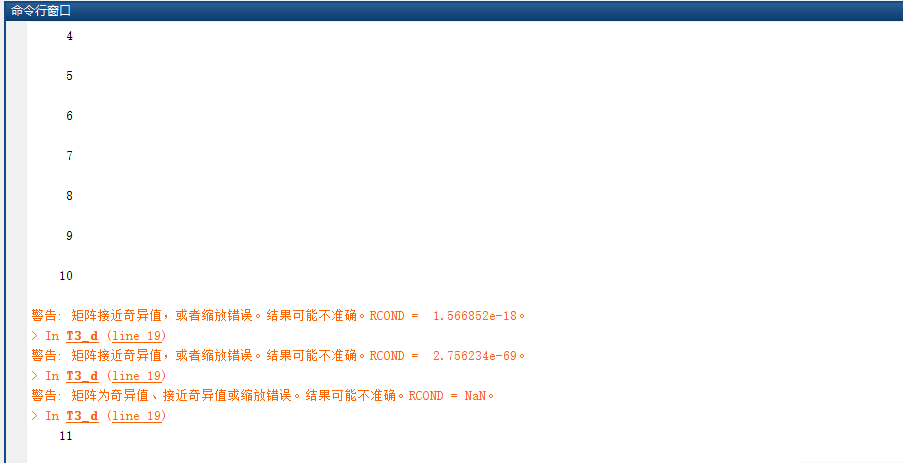
\includegraphics[width=0.6\textwidth]{image/T3_d.png}
	\caption{第三题(d)小题解}
\end{figure}
\end{enumerate}

\end{document}
